\documentclass[10pt]{article}  

%%%%%%%% PREÁMBULO %%%%%%%%%%%%
\title{Plantilla para reportes de proyecto}
\usepackage[spanish]{babel} %Indica que escribiermos en español
\usepackage[utf8]{inputenc} %Indica qué codificación se está usando ISO-8859-1(latin1)  o utf8  
\usepackage{amsmath} % Comandos extras para matemáticas (cajas para ecuaciones,
% etc)
\usepackage{amssymb} % Simbolos matematicos (por lo tanto)
\usepackage{graphicx} % Incluir imágenes en LaTeX
\usepackage{color} % Para colorear texto
\usepackage{subfigure} % subfiguras
\usepackage{float} %Podemos usar el especificador [H] en las figuras para que se
% queden donde queramos
\usepackage{capt-of} % Permite usar etiquetas fuera de elementos flotantes
% (etiquetas de figuras)
\usepackage{sidecap} % Para poner el texto de las imágenes al lado
	\sidecaptionvpos{figure}{c} % Para que el texto se alinie al centro vertical
\usepackage{caption} % Para poder quitar numeracion de figuras
\usepackage{commath} % funcionalidades extras para diferenciales, integrales,
% etc (\od, \dif, etc)
\usepackage{cancel} % para cancelar expresiones (\cancelto{0}{x})
 
\usepackage{anysize} 					% Para personalizar el ancho de  los márgenes
\marginsize{2cm}{2cm}{2cm}{2cm} % Izquierda, derecha, arriba, abajo


\usepackage{appendix}
\renewcommand{\appendixname}{Apéndices}
\renewcommand{\appendixtocname}{Apéndices}
\renewcommand{\appendixpagename}{Apéndices} 

% Para que las referencias sean hipervínculos a las figuras o ecuaciones y
% aparezcan en color
\usepackage[colorlinks=true,plainpages=true,citecolor=blue,linkcolor=blue]{hyperref}
%\usepackage{hyperref} 
% Para agregar encabezado y pie de página
\usepackage{fancyhdr} 
\pagestyle{fancy}
\fancyhf{}
\fancyhead[L]{\footnotesize UAEH} %encabezado izquierda
\fancyhead[R]{\footnotesize Colegio de posgrado}   % dereecha
\fancyfoot[R]{\footnotesize Sistemas Embebidos}  % Pie derecha
\fancyfoot[C]{\thepage}  % centro
\fancyfoot[L]{\footnotesize Maestría en Internet de las Cosas}  %izquierda
\renewcommand{\footrulewidth}{0.4pt}


\usepackage{listings} % Para usar código fuente
\definecolor{dkgreen}{rgb}{0,0.6,0} % Definimos colores para usar en el código
\definecolor{gray}{rgb}{0.5,0.5,0.5} 
% configuración para el lenguaje que queramos utilizar
\lstset{language=Matlab,
   keywords={break,case,catch,continue,else,elseif,end,for,function,
      global,if,otherwise,persistent,return,switch,try,while},
   basicstyle=\ttfamily,
   keywordstyle=\color{blue},
   commentstyle=\color{red},
   stringstyle=\color{dkgreen},
   numbers=left,
   numberstyle=\tiny\color{gray},
   stepnumber=1,
   numbersep=10pt,
   backgroundcolor=\color{white},
   tabsize=4,
   showspaces=false,
   showstringspaces=false}

\newcommand{\sen}{\operatorname{\sen}}	% Definimos el comando \sen para el seno
%en español

\title{Plantilla de proyecto final}
% Basada en la plantilla para reportes UPIITA de  Overleaf

%%%%%%%% TERMINA PREÁMBULO %%%%%%%%%%%%

\begin{document}

%%%%%%%%%%%%%%%%%%%%%%%%%%%%%%%%%% PORTADA %%%%%%%%%%%%%%%%%%%%%%%%%%%%%%%%%%%%%%%%%%%%
																					%%%
\begin{center}																		%%%
\newcommand{\HRule}{\rule{\linewidth}{0.5mm}}									%%%\left
 																					%%%
\begin{minipage}{0.48\textwidth} \begin{flushleft}

\includegraphics[scale = 0.25]{Imagenes/uaeh.png}
\end{flushleft}\end{minipage}
\begin{minipage}{0.48\textwidth} \begin{flushright}

\includegraphics[scale = 0.25]{Imagenes/colpos2.png}
\end{flushright}\end{minipage}

													 								%%%
\vspace*{1.0cm}								%%%
																					%%%	
\textsc{\huge Universidad Autónoma del Estado de\\ \vspace{5px}Hidalgo}\\[1.5cm]	

\textsc{\LARGE Colegio de Posgrado }\\[1.5cm]													%%%

\begin{minipage}{0.9\textwidth} 
\begin{center}																					%%%
\textsc{\LARGE Sistemas Embebidos }
\end{center}
\end{minipage}\\[0.5cm]
%%%
    																				%%%
 			\vspace*{1cm}																		%%%
																					%%%
\HRule \\[0.4cm]																	%%%
{ \huge \bfseries Plataforma Digital Automatizada de Transporte Público}\\[0.4cm]	%%%
 																					%%%
\HRule \\[1.5cm]																	%%%
 																				%%%
																					%%%
\begin{minipage}{0.46\textwidth}													%%%
\begin{flushleft} \large															%%%

% Aqui a continuación pongan los nombres de los integrantes
\emph{Nombre del alumno:}\\	
Erick Renato Vega Cerón \\

%%%
			%\vspace*{2cm}	
            													%%%
										 						%%%
\end{flushleft}																		%%%
\end{minipage}		
																%%%
\begin{minipage}{0.52\textwidth}		
\vspace{-0.6cm}											%%%
\begin{flushright} \large															%%%
\emph{Profesor:} \\																	%%%
Dr. Ismael Domínguez Jiménez.\\
													%%%
\end{flushright}																	%%%
\end{minipage}	
\vspace*{1cm}
%\begin{flushleft}
 	
%\end{flushleft}
%%%
 		% \flushleft{\textbf{\Large Nombre del curso (IMEC XXZZ)}	}\\																		%%%
\vspace{2cm} 																				
\begin{center}	
Torre de posgrado - Ciudad del Conocimiento \\
{\large \today}																	%%%
 			\end{center}												  						
\end{center}							 											
																					
\newpage																		
%%%%%%%%%%%%%%%%%%%% TERMINA PORTADA %%%%%%%%%%%%%%%%%%%%%%%%%%%%%%%%

\tableofcontents 

\newpage

\section{Resumen.}




``Cahuitl'' destaca como una prueba de concepto innovadora, implementando un sistema integral de automatización de rutas y gestión digital de pagos en el transporte público. La integración de tecnologías de Internet de las Cosas en hardware embebido incluye la recopilación de datos no solo del sensor DHT11 sino también de un sensor GPS. Estos datos se transmiten a una Computadora de Placa Única (SBC), que utiliza Edge Computing para el procesamiento y la presentación. Este progreso establece las bases tecnológicas esenciales para desarrollar un prototipo funcional, con el propósito de optimizar el sistema de transporte público y avanzar hacia una ciudad más sostenible.
\cite{IEEEreferencias:Ref1}
\cite{IEEEreferencias:Ref2}




\section{Introducción.} 


*


\section{Problema a resolver}

Según datos del INEGI de 2015, de los 557,093 habitantes aproximados en la Zona Metropolitana de Pachuca, alrededor de 67,874 personas trabajan o estudian en otro municipio, dependiendo del transporte público para desplazarse a sus lugares correspondientes. En la actualidad, los usuarios del transporte público en la ZMP enfrentan largos tiempos de espera y desconocen por completo las rutas disponibles. Además, los conductores deben encargarse del cobro de pasajes, la gestión de tiempos de ruta y la conducción del vehículo, lo que afecta la calidad del servicio y disminuye la adopción del transporte público, agravando la problemática. 
\cite{IEEEreferencias:Ref4}

\section{Propuesta de Solución}
Para abordar estos desafíos, la gestión de rutas, el cobro automatizado y la recolección de datos operativos se destacan como soluciones clave. Ejemplo de estas implementaciones son los casos en Ciudad de México o Guadalajara, donde el cobro automatizado y la gestión de rutas ya se han implementado en el transporte masivo. La implementación de tecnologías que optimicen las rutas, reduzcan los tiempos de espera, simplifiquen los pagos y mejoren la certeza del servicio para los usuarios puede revitalizar la confianza en el transporte público. La recopilación y análisis de datos permiten una toma de decisiones más informada, contribuyendo así a un sistema de transporte más eficiente y atractivo para los viajeros.
\cite{IEEEreferencias:Ref5}
\cite{IEEEreferencias:Ref6}

\section{Objetivo}
Haec quae dicis admodum in omni tempore semper cómoi tu dicas dicere. Et ne forte dicant quod duplex est. Plurrimi maximus res est cogitans in quam solvitur quaestio satis perspicuum parcentes nulla divisio requiritur moralis accurate perpensis omnibus iudiciis et certa . Electus quisque valet mensura .

\subsection{Objetivos especificos}
\begin{enumerate}
    \item Haec quae dicis admodum in omni tempore semper cómoi tu dicas dicere. Et ne forte dicant quod duplex est. Plurrimi maximus res est cogitans in quam solvitur quaestio satis perspicuum parcentes nulla divisio requiritur mora
    \item lis accurate perpensis omnibus iudiciis et certa . Electus quisque valet mensura .
    \item Haec quae dicis admodum in omni tempore semper cómoi tu dicas dicere. Et ne forte 

\end{enumerate}


\section{Material a utilizar}
aec quae dicis admodum in omni tempore semper cómoi tu dicas dicere. Et ne forte dicant quod duplex est. Plurrimi max
   \begin{enumerate}
    \item Haec quae dicis admodum in omni tempore semper cómoi tu dicas dicere. Et ne forte dicant quod duplex est. Plurrimi maximus res est cogitans in quam solvitur quaestio satis perspicuum parcentes nulla divisio requiritur mora
    \item lis accurate perpensis omnibus iudiciis et certa . Electus quisque valet mensura .
    \item Haec quae dicis admodum in omni tempore semper cómoi tu dicas dicere. Et ne forte 
   \end{enumerate}

\section{Procedimiento realizado}

Haec quae dicis admodum in omni tempore semper cómoi tu dicas dicere. Et ne forte dicant quod duplex est. Plurrimi maximus res est cogitans in quam solvitur quaestio satis perspicuum parcentes nulla divisio requiritur moralis accurate perpensis omnibus iudiciis et certa . Electus quisque valet mensura .
Haec quae dicis admodum in omni tempore semper cómoi tu dicas dicere. Et ne forte dicant quod duplex est. Plurrimi maximus res est cogitans in quam solvitur quaestio satis perspicuum parcentes nulla divisio requiritur moralis accurate perpensis omnibus iudiciis et certa . Electus quisque valet mensura .
Haec quae dicis admodum in omni tempore semper cómoi tu dicas dicere. Et ne forte dicant quod duplex est. Plurrimi maximus res est cogitans in quam solvitur quaestio satis perspicuum parcentes nulla divisio requiritur moralis accurate perpensis omnibus iudiciis et certa . Electus quisque valet mensura .


\subsection{Diagrama a bloques}
iudiciis et certa . Electus quisque valet mensura .
Haec quae dicis admodum in omni tempore semper cómoi tu dicas dicere. Et ne forte dicant quod duplex est. Plurrimi maximus res est cogitans in quam solvitur quaestio satis perspicuum parcentes nulla divisio requiritur moralis accurate p
\begin{figure}[H]
	\begin{center}
 		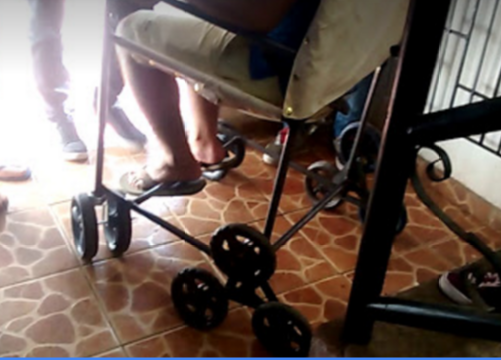
\includegraphics[width = 0.5\textwidth]{Imagenes/silla3ruedas}
 		\captionof{figure}{\label{fig:silla3ruedas}Silla de ruedas para subir escaleras} 
	\end{center} 
\end{figure}



\subsection{Implentación del prototipo.}


Describa los resultados obtenidos. 



Haec quae dicis admodum in omni tempore semper cómoi tu dicas dicere. Et ne forte dicant quod duplex est. Plurrimi maximus res est cogitans in quam solvitur quaestio satis perspicuum parcentes nulla divisio requiritur moralis accurate perpensis omnibus iudiciis et certa . Electus quisque valet mensura .
Haec quae dicis admodum in omni tempore semper cómoi tu dicas dicere. Et ne forte dicant quod duplex est. Plurrimi maximus res est cogitans in quam solvitur quaestio satis perspicuum parcentes nulla divisio requiritur moralis accurate perpensis omnibus iudiciis et certa . Electus quisque valet mensura .
Haec quae dicis admodum in omni tempore semper cómoi tu dicas dicere. Et ne forte dicant quod duplex est. Plurrimi maximus res est cogitans in quam solvitur quaestio satis perspicuum parcentes nulla divisio requiritur moralis accurate perpensis omnibus iudiciis et certa . Electus quisque valet mensura .

Haec quae dicis admodum in omni tempore semper cómoi tu dicas dicere. Et ne forte dicant quod duplex est. Plurrimi maximus res est cogitans in quam solvitur quaestio satis perspicuum parcentes nulla divisio requiritur moralis accurate perpensis omnibus iudiciis et certa . Electus quisque valet mensura .
Haec quae dicis admodum in omni tempore semper cómoi tu dicas dicere. Et ne forte dicant quod duplex est. Plurrimi maximus res est cogitans in quam solvitur quaestio satis perspicuum parcentes nulla divisio requiritur moralis accurate perpensis omnibus iudiciis et certa . Electus quisque valet mensura .




\section{Conclusiones.}

Explique por qué su diseño sirve (o nó) y qué hace falta por hacer.
Responda las expectativas generadas en la Introducción.
Analice sus resultados críticamente y diga si son creíbles y responda qué tan seguras son sus propuestas. 



%%%%%%% Bibliografía %%%%%%%%
\bibliographystyle{bst/IEEEtran.bst} 
\addcontentsline{toc}{section}{Referencias}  
\bibliography{bib/IEEEabrv.bib/IEEEreferencias.bib} 
%%%%%%% Bibliografía %%%%%%%%    



\end{document}